\section{Auswertung}

Fehler und Ausgleichsrechnungen werden mit den Python-Paketen SciPy \cite{scipy} und uncertainties \cite{uncertain} berechnet.

\subsection{Untergrundsubtraktion}

\begin{figure}[htp]
    \centering
    \begin{subfigure}[t]{0.5\textwidth}
        \centering
        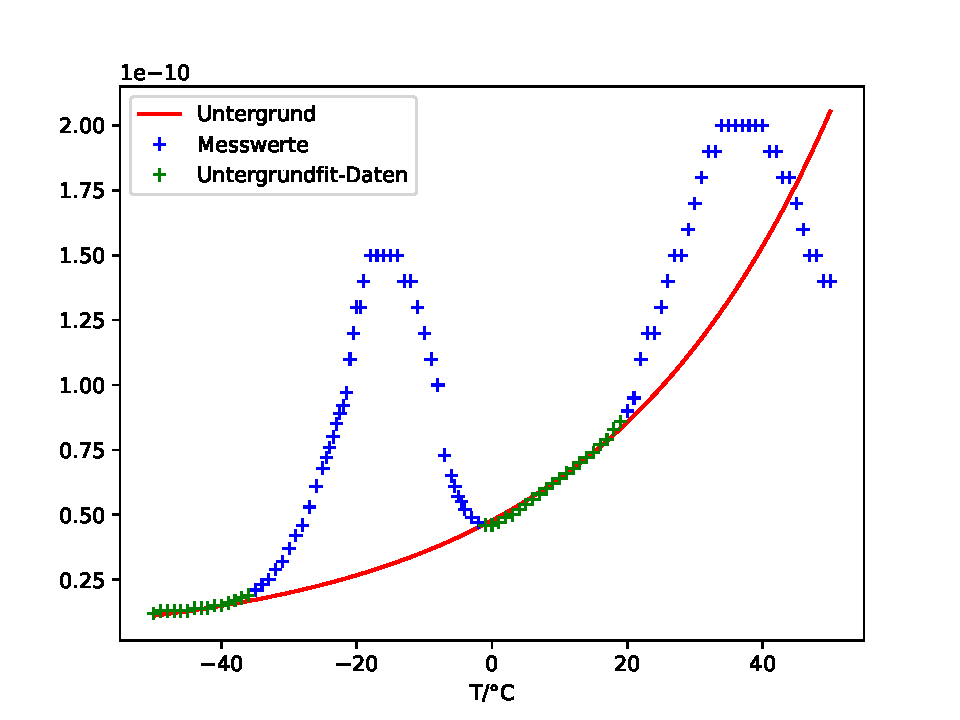
\includegraphics[width=\textwidth]{img/heizrate_15C.pdf}
        \caption{Heizrate: $\SI{1.5}{\kelvin\per\second}$}
    \end{subfigure}%
    ~
    \begin{subfigure}[t]{0.5\textwidth}
        \centering
        \includegraphics[width=\textwidth]{img/heizrate_2C.pdf}
        \caption{Heizrate: $\SI{2}{\kelvin\per\second}$}
    \end{subfigure}
    \caption{Temperaturabhängiger Verlauf der Messdaten und Fit an den Untergrund durch ein Polynom fünften Grades.}
\end{figure}

\begin{figure}[htp]
    \centering
    \begin{subfigure}[t]{0.5\textwidth}
        \centering
        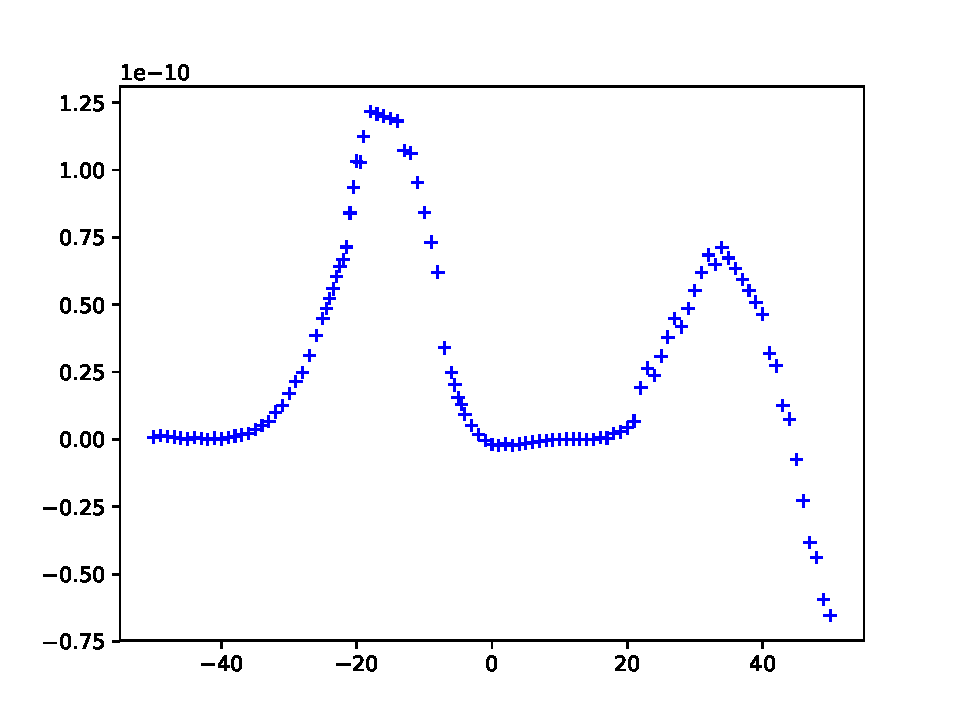
\includegraphics[width=\textwidth]{img/heizrate_15C_no-bg.pdf}
        \caption{Heizrate: $\SI{1.5}{\kelvin\per\second}$}
    \end{subfigure}%
    ~
    \begin{subfigure}[t]{0.5\textwidth}
        \centering
        \includegraphics[width=\textwidth]{img/heizrate_2C_no-bg.pdf}
        \caption{Heizrate: $\SI{2}{\kelvin\per\second}$}
    \end{subfigure}
    \caption{Vom Untergrund bereinigte und Messwerte ohne den zweiten Anstieg des Relaxationsstroms.}
\end{figure}

Heizrate: 1.5 K/s
Background Fit:
a = (6.3+/-1.3)e-18
b = (-6.2+/-1.4)e-15
c = (2.3+/-0.5)e-12
d = (-3.8+/-0.9)e-10
e = (2.4+/-0.6)e-08
Einfacher linearer Fit für W:
a = (-1.388+/-0.033)e+04
b = 32.1+/-1.4
Aktivierungsenergie W = 1.196+/-0.029 eV
Relaxationszeit tau0 = (0.7+/-1.0)e-23 s
Linearer Fit an Integral für W:
a = (1.022+/-0.034)e+04
b = -37.3+/-1.4
Aktivierungsenergie W = 0.880+/-0.029 eV
Relaxationszeit tau0 = (1.7+/-2.4)e-17 s

Heizrate: 2 K/s
Background Fit:
a = (1.23+/-0.22)e-17
b = (-1.20+/-0.23)e-14
c = (4.4+/-0.9)e-12
d = (-7.1+/-1.5)e-10
e = (4.3+/-0.9)e-08
Einfacher linearer Fit für W:
a = (-9.61+/-0.30)e+03
b = 15.0+/-1.2
Aktivierungsenergie W = 0.829+/-0.026 eV
Relaxationszeit tau0 = (2.7+/-3.2)e-16 s
Linearer Fit an Integral für W:
a = (1.011+/-0.018)e+04
b = -36.8+/-0.7
Aktivierungsenergie W = 0.871+/-0.015 eV
Relaxationszeit tau0 = (3.8+/-2.6)e-17 s

\subsection{Bestimmung der Aktivierungsenergie durch einen linearen Fit}

\begin{figure}[htp]
    \centering
    \begin{subfigure}[t]{0.5\textwidth}
        \centering
        \includegraphics[width=\textwidth]{img/hr15_W-aus-Methode1.pdf}
        \caption{Heizrate: $\SI{1.5}{\kelvin\per\second}$}
    \end{subfigure}%
    ~
    \begin{subfigure}[t]{0.5\textwidth}
        \centering
        \includegraphics[width=\textwidth]{img/hr2_W-aus-Methode1.pdf}
        \caption{Heizrate: $\SI{2}{\kelvin\per\second}$}
    \end{subfigure}
    \caption{Bestimmung der Aktivierungsenergie $W$ durch einen linearen Fit an den Anstieg des Relaxationsstroms.}
\end{figure}

\subsection{Bestimmung der Aktivierungsenergie durch Integration}

\begin{figure}[htp]
    \centering
    \begin{subfigure}[t]{0.5\textwidth}
        \centering
        \includegraphics[width=\textwidth]{img/hr15_W-aus-Methode2.pdf}
        \caption{Heizrate: $\SI{1.5}{\kelvin\per\second}$}
    \end{subfigure}%
    ~
    \begin{subfigure}[t]{0.5\textwidth}
        \centering
        \includegraphics[width=\textwidth]{img/hr2_W-aus-Methode2.pdf}
        \caption{Heizrate: $\SI{2}{\kelvin\per\second}$}
    \end{subfigure}
    \caption{Bestimmung der Aktivierungsenergie $W$ durch einen linearen Fit an die gewichtete Integration des gesamten Verlaufs des Relaxationsstroms.}
\end{figure}

Eine genauere Bestimmung der Aktivierungsenergie $W$ erfolgt anhand der Gleichung
\begin{equation*}
    F(T) = \frac{\int_T^{T^\ast} i(T^\prime)\mathrm{d}T^\prime}{i(T)}\,.
\end{equation*}
Dazu wird $F(T)$ linear gegen $1/T$ aufgetragen:
\begin{equation*}
    F(T) = a \cdot\frac{1}{T} + b\,,
\end{equation*}
die Aktivierugnsenergie ist dann
\begin{equation*}
    W = a \cdot k_\text{B}\,.
\end{equation*}
Die Relaxationszeit $\tau_0$ wird mit die Lage des maximalen Stroms $T_\text{max}$ bestimmt, hier fehlt noch eine genauere Beschreibung, wie man zu dieser Gleichung kommt:
\begin{equation}
    \label{eqn:tau0}
    \tau_0 = \frac{k_\text{B}T_\text{max}^2}{Wb}
             \exp\!\left[-\frac{W}{k_\text{B}T_\text{max}} \right]
\end{equation}
